\documentclass{article} % This line defines the type of document. 'article' is a common class for small documents.
\usepackage[margin=1in]{geometry}
\usepackage{graphicx}

\begin{document} % This line marks the beginning of the document content.


\noindent\makebox[\linewidth]{\rule{\textwidth}{1pt}} 
\vspace*{0mm} % adds vertical space before the title
\begin{center}
    \Large\textbf{Toy Models of Superposition Replication and Findings}
\end{center}
\vspace*{2mm} % adds vertical space before the title
\noindent\makebox[\linewidth]{\rule{\textwidth}{1pt}}
\newline

\begin{abstract}
\begin{quote}
    Lorem ipsum dolor sit amet, consectetur adipiscing elit. Aliquam eu neque 
    vitae velit efficitur venenatis. Fusce nec sem mauris. Fusce molestie massa 
    et dolor euismod, ut pharetra urna tristique. Vestibulum vel tincidunt erat. 
    Nam efficitur mi sed eros dictum elementum. Phasellus posuere felis euismod, 
    volutpat nulla sit amet, efficitur ipsum. Mauris ut eros in nisl placerat 
    finibus a non mi. Integer a porttitor mauris. Sed a lacus vel nulla lacinia 
    pretium at vel tellus. Vivamus pharetra ipsum sed erat hendrerit placerat. 
    Mauris id mauris convallis, lobortis dui in, pulvinar turpis. Aliquam erat 
    volutpat. Vivamus facilisis pharetra nunc fermentum blandit. Donec vehicula 
    dictum libero, vitae consequat neque tempor in.
\end{quote}
\end{abstract}

\begin{figure}[h]
    \centering
    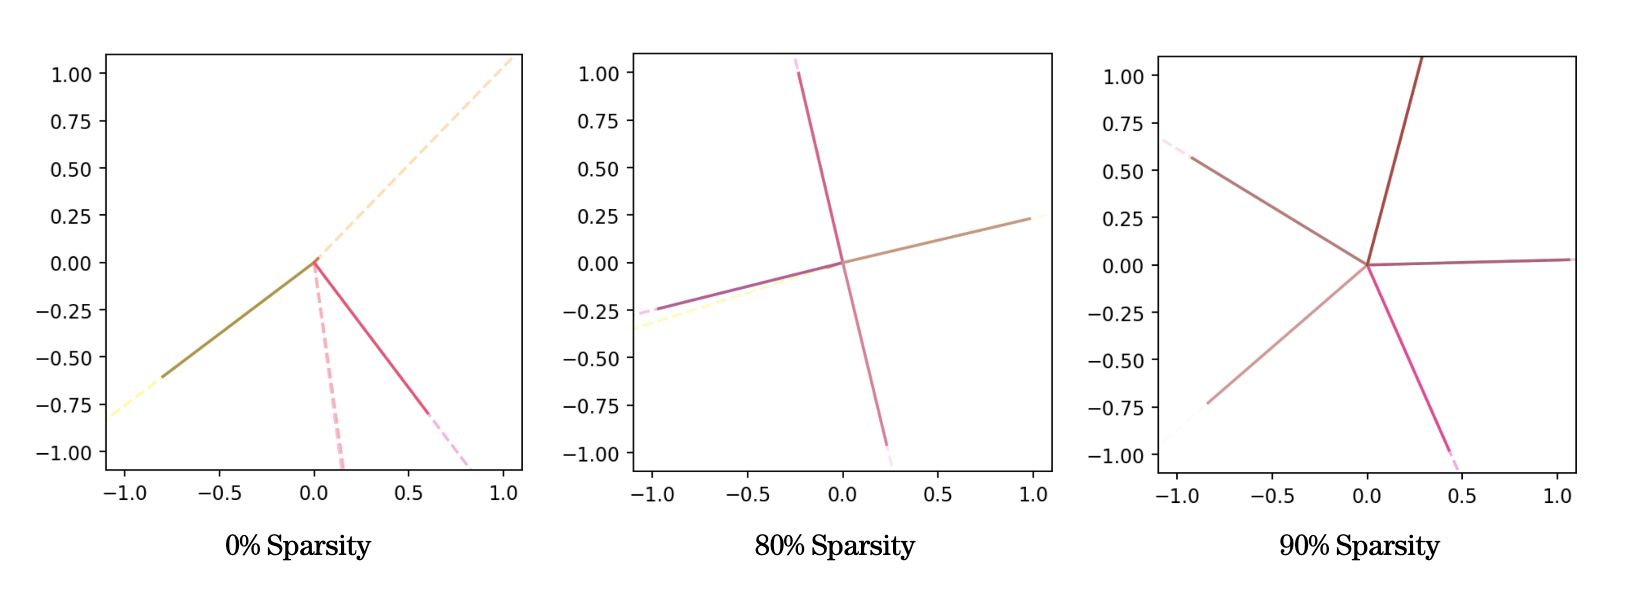
\includegraphics[width=0.7\linewidth]{section_1/images/section1_replicated_graphic.png}
    \caption{Caption for the image.}
    \label{fig:my_label}
\end{figure}

\begin{figure}[h]
    \centering
    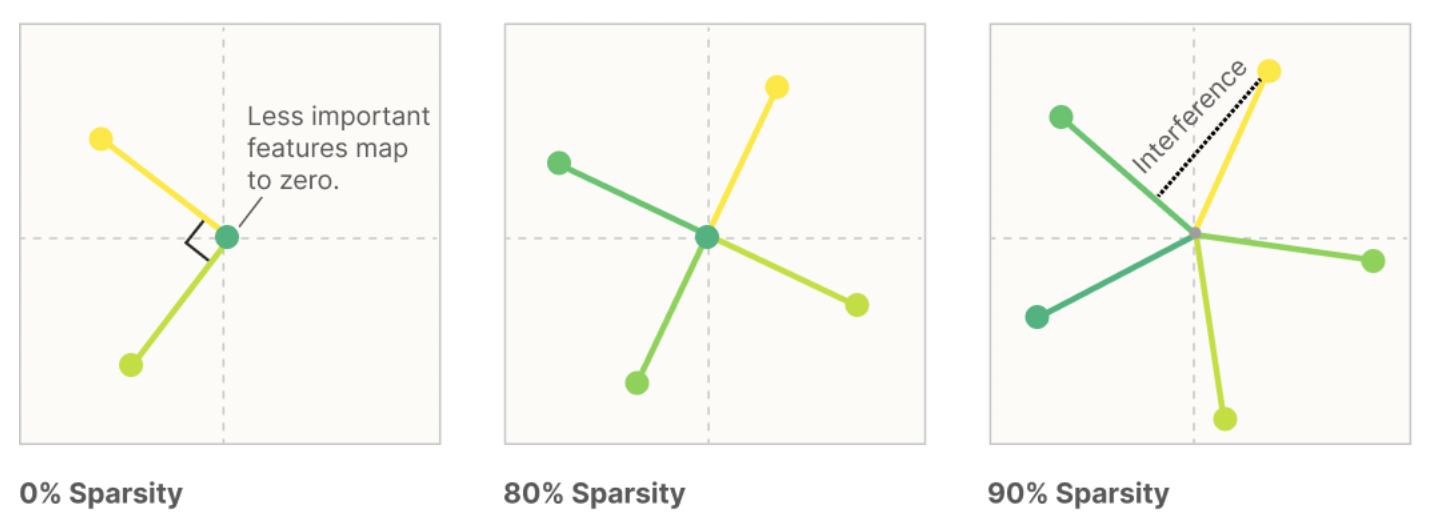
\includegraphics[width=0.67\linewidth]{section_1/images/section1_anthropic_graphic_.png}
    \caption{Caption for the image.}
    \label{fig:my_label}
\end{figure}


% Hello World! % Your content goes here.

\end{document} % This line marks the end of the document content.